\section{Problem Statement and Modeling}
\label{sec:problem-model}

We formalize our SD acquisition as a \emph{graph crawling problem}. We show that a relaxed version thereof is NP-hard, even if the website is
known before the crawl (it is not!) in
Sec.~\ref{section:problem_statement}. Then we detail the mapping of our problem into the graph crawling framework, including a crucial choice of labels for the graph edges, in Sec.~\ref{section:graph_to_website}.

\subsection{Graph Crawling Problem}
\begin{toappendix}
	\begin{figure}[h]
		\centering
		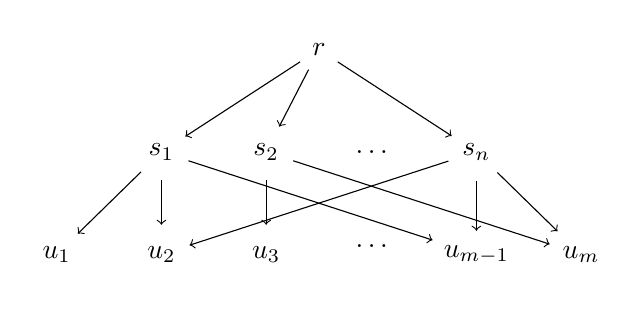
\begin{tikzpicture}[level distance=1cm,
				level 1/.style={sibling distance=5cm},
				level 2/.style={sibling distance=2.5cm}]

			\node[circle] (root) {$r$};
			\node[circle] (s1) at (-2,-1.3) {$s_1$};
			\node[circle] (s2) at (-0.67,-1.3) {$s_2$};
			\node at (0.67,-1.3) {$\dots$};
			\node[circle] (sn) at (2,-1.3) {$s_n$};

			\draw[->] (root) -- (s1);
			\draw[->] (root) -- (s2);
			\draw[->] (root) -- (sn);

			\node[circle] (a1) at (-3.33,-2.6) {$u_1$};
			\node[circle] (a2) at (-2,-2.6) {$u_2$};
			\node[circle] (a3) at (-0.67,-2.6) {$u_3$};
			\node at (0.67,-2.5) {$\dots$};
			\node[circle] (am1) at (2,-2.6) {$u_{m-1}$};
			\node[circle] (am) at (3.33,-2.6) {$u_m$};

			\draw[->] (s1) -- (a1);
			\draw[->] (s1) -- (a2);
			\draw[->] (s1) -- (am1);

			\draw[->] (s2) -- (a3);
			\draw[->] (s2) -- (am);

			\draw[->] (sn) -- (a2);
			\draw[-] (sn) -- ++(0,-1) coordinate (extended) -- (am1);
			\draw[->] (sn) -- (extended);
			\draw[->] (sn) -- (am);

		\end{tikzpicture}
		\caption{Graphical summarization of the graph $G_{\textrm{sc}}$}
		\label{fig:graph_set_cover}
	\end{figure}

	\subsection{Graph Crawling Problem}
\end{toappendix}
\label{section:problem_statement}

We model a website
as a rooted,
node-weighted, edge-labeled directed graph. Each node represents a webpage, and each edge is a hypertext link leading from one to another.
We fix a countable set~$\mathcal{L}$ of labels, e.g., finite sequences of
character strings.

% lax begin Lax117614.WebsiteGraphs
\begin{definition}
	A \emph{website graph} is a tuple $G = (V, E, r, \omega, \lambda)$, with: $V$ a finite set of \emph{nodes}
	(representing webpages);
	$E\subseteq V^2$ a set of \emph{edges} (representing hyperlinks);
	$r \in V$ the \emph{root} of the graph (the input webpage);
	$\omega: V\to\mathbb{R}^+$ a \emph{cost} function assigning a positive
	weight to every node (the cost of	retrieving that page);
	$\lambda: E\to\mathcal{L}$ a \emph{labeling} function, assigning a label to	each link found in a page.
\end{definition}
% lax end

% lax begin Lax117614.GraphCrawlingProblem
On such a graph, we define a \emph{crawl}
and its \emph{cost} as follows:
\begin{definition}
	A \emph{crawl} of a website graph $G$
	is an $r$-rooted subtree $T=(V',E')$ of $(V,E)$.
	Its total cost, $\omega(T)$, is defined as $\sum_{\substack{u\in V'}} \omega(u)$.
\end{definition}

The graph crawling problem is formalized as follows:

\begin{problem}
\label{problem:graph-crawling}
Given a website graph $G=(V,E,R,\omega,\lambda)$ and a subset~$V^*$
of \emph{targets} in~$V$
, the graph crawling problem is to find a crawl $T=(V',E')$ of~$G$ with $V^*\subseteq V'$, of minimal total cost.
\end{problem}
% lax end

We define the \emph{frontier} of a crawl $\left\{u\in V\setminus V'\mid
\left(v,u\right)\in E, v\in V'\right\}$: nodes that have not
been crawled but are pointed to from nodes that have been. Figure~\ref{fig:example_graph_crawling} shows a website graph as well as a possible crawl and its frontier. Even assuming the graph is fully known in advance, the graph crawling problem is intractable:

% lax begin Lax117614.GraphCrawlingNPComplete
\begin{propositionrep}
	\label{prop:np-complete}
	Given a website graph $G=(V,E,r,\omega,\lambda)$, a subset
	$V^*\subseteq V$ and some $B\in\mathbb{R}^+$, determining
	whether there exists a crawl~$T=(V',E')$ of $G$ such that $V^*\subseteq V'$
	and $\omega(T)\leq B$ is
	NP-complete; hardness holds even when $\omega$ is a constant function.
  This holds even when nodes in $V^*$ do not have any out 
    links in~$G$.
\end{propositionrep}
% lax end

This is the decision variant of the graph crawling problem. Hardness
is shown by reduction from the set cover problem~\cite{johnson1979computers2}; the proof can be found in the extended version in~\cite{github_repository}.
\begin{figure}
	\centering
	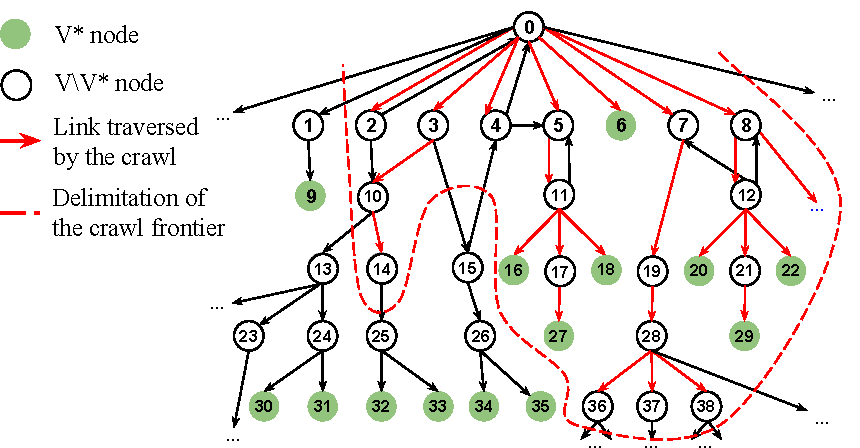
\includegraphics[width=\linewidth]{plots/example_graph_crawling.pdf}
	\caption{Sample website, crawl, and frontier}
	\label{fig:example_graph_crawling}
\end{figure}

\begin{proof}
% lax begin Lax117614Proofs.Bridge.graphCrawling_NP_complete
	To show NP-completeness, we must show that the problem belongs to NP and is NP-hard.

	Let us start with the upper bound. Given a graph
	$G=(V,E,r,\omega,\lambda)$, we guess a subgraph $T=(V',E')$ of~$G$
	(which is a polynomial-sized guess). In polynomial time, we check
	whether $T$ is a $r$-rooted tree (i.e., whether it is connected,
	includes~$r$, $r$ has indegree 0 and other nodes indegree 1), we
	check that $V'$ contains all nodes of $V^*$, and we check that
	$\omega(T)\leq B$. We accept if and only if these conditions are
	all satisfied. This yields a nondeterministic polynomial-time
	algorithm, meaning the problem is in NP.

	We now move to the lower bound.
	Our
	crawling problem can be seen as a directed variant of the well-known
	NP-complete \emph{Steiner Tree} \cite{johnson1979computers}
	problem. NP-hardness of the directed Steiner tree problem is mentioned in
	the literature (see, e.g., \cite{watel2016greedy}), but as it is not
	formally shown there, we prefer for completeness of the presentation
% lax begin Lax799700.SetFamily
	reducing from the set cover problem, a classic NP-hard
	problem~\cite{johnson1979computers}.
% lax end
	We denote $\mathcal{U} =
		\left\{u_1, \dots, u_m\right\}$ a set of $m$ elements called the
	universe. We also define a collection $\mathcal{S} = \left\{s_1,
		\dots, s_n\right\}$ of $n$ non-empty subsets, each of them containing some elements of $\mathcal{U}$, such that:
	\[
		\bigcup_{s \in \mathcal{S}} s = \mathcal{U}.
	\]
	In its decision version, the set cover consists in given such a
	universe and collection, given a natural integer~$B$, determining
	whether there exists a \emph{cover} $\mathcal{C} \subseteq
		\left\{s_1, \dots, s_n\right\}$ such that $\left\lvert\mathcal{C}\right\rvert \leq B$ and:
	\[
		\bigcup_{s \in \mathcal{C}} s = \mathcal{U}.
	\]
	\def\sc{\mathrm{sc}}

	We now propose a polynomial-time many-one reduction of the set cover problem to an instance of
	the graph crawling problem. We create a website graph
	$G_\sc = \left(V_\sc, E_\sc, r, \omega,
		\lambda\right)$ as follows. We set $V_\sc$ to be
	$\{\,u_1,\dots,u_m,r,s_1,\dots,s_n\,\}$, including representations for
	every element of the universe~$\mathcal{U}$, every set of the
	collection~$\mathcal{S}$, as well as a distinct root~$r$ (by abuse of
	notation, we do not distinguish between elements of $\mathcal{U}$,
	$\mathcal{S}$ and the way they are represented in~$V_\sc$).
	We define $E_\sc$ as $\left\{\left(r, s_i\right) \, |
		\, i \in \left\{1, \dots, n\right\}\right\} \cup \left\{\left(s_i,
		u\right) \, | \, u \in s_i, i \in \left\{1, \dots, n\right\}\right\}$.
	In other words, in $G_\sc$ from the origin
	(root) $r$, we model each element of $\mathcal{S}$ as a vertex, that
	can be reached following a dedicated (directed) edge. Finally, for
	each new vertex $s_i \in \mathcal{S}$, we have as many outgoing edges
	as there are elements of $\mathcal{U}$ in $s_i$. Finally, we set
	$\omega$ to be the constant function that assigns cost~$1$ to every
	vertex, and $\lambda$ to be some constant function.
	The result is a graph in the form of a tree of depth 2, depicted in
	Figure~\ref{fig:graph_set_cover}. We fix $V^*$ to be
  $\mathcal{U}$. Observe that nodes in $\mathcal{U}$ do not have
  any outgoing links. We state that there exists
	$\mathcal{C} \subseteq \left\{s_1, \dots, s_n\right\}$ such that
	$\left\lvert \mathcal{C} \right\rvert \leq B$ and $\bigcup_{i \in
			\mathcal{C}} s_i = \mathcal{U}$ if and only if there exists a crawl
	$T_\sc$ of $G_\sc$ containing all elements of $V^*$ and of total cost
	$\omega(T_\sc) \leq \left\lvert \mathcal{U} \right\rvert + B + 1$.

	Let us explain why this reduction is
	polynomial-time. In set cover, the universe $\mathcal{U}$ can be
	described by the number $m$ of its elements, with representation size
	$\Theta(\log m)$. Each set of $\mathcal{S}$ needs to list every element
	within this set, so a set $s_i$ has representation size $\Theta(\log
		m\times |s_i|)$. Finally, $B$ has representation size $\Theta(\log B)$.
	This yields a total input size of $\Theta((\log
		m)\left(\sum_{i=1}^n|s_i|+1\right)+\log B)$. Note that $\sum_{i=1}^n
		|s_i|\geq \max(m,n)$ so this is $\Omega(\max(m,n)\log m+\log B)$.
	But then, the construction depicted in
	Figure~\ref{fig:graph_set_cover} can clearly be done in time
	polynomial in $m$ and $n$ (namely, in $O(m\times n)$ in the
	worst case where every set of the collection contains every element).
	The reduction is therefore polynomial-time.

	We now proceed to show equivalence between the initial problem known
	to be NP-hard (set cover) and the graph crawling instance presented
	above. First, suppose that
	there exists $\mathcal{C} \subseteq \left\{s_1, \dots,
		s_n\right\}$ such that $\left\lvert \mathcal{C} \right\rvert \leq B$
	and $\bigcup_{i \in \mathcal{C}} s_i = \mathcal{U}$.
	Then consider the crawl $T_\sc$ of $G_\sc$ formed by including
	$r$, every element of
	$\mathcal{C}$ using the edge from $r$ to that element, and every
	edge from an element of $\mathcal{C}$ to an element of $\mathcal{U}$.
	Since $\mathcal{C}$ is a cover, this includes all elements of
	$\mathcal{U}$. The total cost of this crawl
	$\omega(T_\sc)=1+|\mathcal{C}|+|\mathcal{U}|\leq |\mathcal{U}|+B+1$.

	Now suppose that there exists a crawl $T_\sc$ of $G_{\textrm{sc}}$ of
	total cost $\omega(T_\sc) \leq \left\lvert \mathcal{U} \right\rvert
		+ B + 1$. Note that by definition of $\omega$, the cost is just the
	number of nodes in $T_\sc$, and this crawl necessarily includes the
	root~$r$ as well as all vertices of $\mathcal{U}$. The remaining
	$\leq B$ vertices are therefore vertices of~$\mathcal{S}$. We pose
	$\mathcal{C}$ to be those. Then $|\mathcal{C}|\leq B$ and since
	$T_\sc$ is a crawl, for every $u\in\mathcal{U}$, there exists at
	least one $s\in\mathcal{C}$ such that the edge $(s,u)$ is in $T_\sc$,
	meaning that $u\in s$. We indeed have
	$\mathcal{U}=\bigcup_{s\in\mathcal{C}} s$.
% lax end
\end{proof}
Optimal methods being out of
reach (websites may have millions of
pages),
we need heuristic methods with a low cost in practice.
